\chapter{Problem analysis}
Our first step will be to define what will the application do and also who will be able to use it.
For this reason we will identify user roles, specify use cases and describe those via use case scenarios.
The output of this chapter is a list of user requirements which will be important in the next chapter.
This analysis is inspired by interviewing a restaurant\footnote{\url{https://www.pizzabudca.sk}  \label{fnlabel}} employee and also two former restaurant\footnote{\url{https://www.sokolzabreh.cz/hospudka}  \label{fnlabel}} owners.

\section{Target group}
The application will focus on restaurants and their guests in the European Union.
The reason behind this is that the EU enforces restaurants to inform their guests about allergens contained in the food they serve, and has already established rules for how to do it.
We would like for the application to be usable internationally, so it needs to have its user interface translated into different languages.
For this purpose we will choose the English, Slovak and Czech languages with the possibility of adding more translations in the future.

\section{User roles}
There are two types of users who will come in contact with the application.
The first type is a \textbf{restaurant}, more specifically its employee who is responsible for creating menus.
This user needs to have a basic understanding of how to use a web browser either on a computer or on a smartphone.
The application will allow restaurant employees to create menus online and will help them with specifying allergens contained in menu items.

The second type of user is a restaurant \textbf{guest}.
They, too, need to have a basic understanding of how to use a web browser either on a computer or on a smartphone.
The application will enable a restaurant guest to create a personal profile where they will specify their food preferences, including the allergies they have and the diets they are on.
When a guest will view a restaurant's menu using the application, the displayed menu will be adapted to meet the guest's profile preferences.
The application will thus make it easier for the guest to choose what they would like to order in a particular restaurant.

\section{Use cases}
Now we are going to depict goals of users which the application will make achievable.
Figure 2.1 contains a use case diagram of the application.
A use case styled with a bold border groups together more use cases and will be expanded further.
All use cases will be structurally described by independent use case scenarios.
A structured use case will contain a description if the goal of a user is not entirely clear from the use case's name.

\begin{figure}[h]
  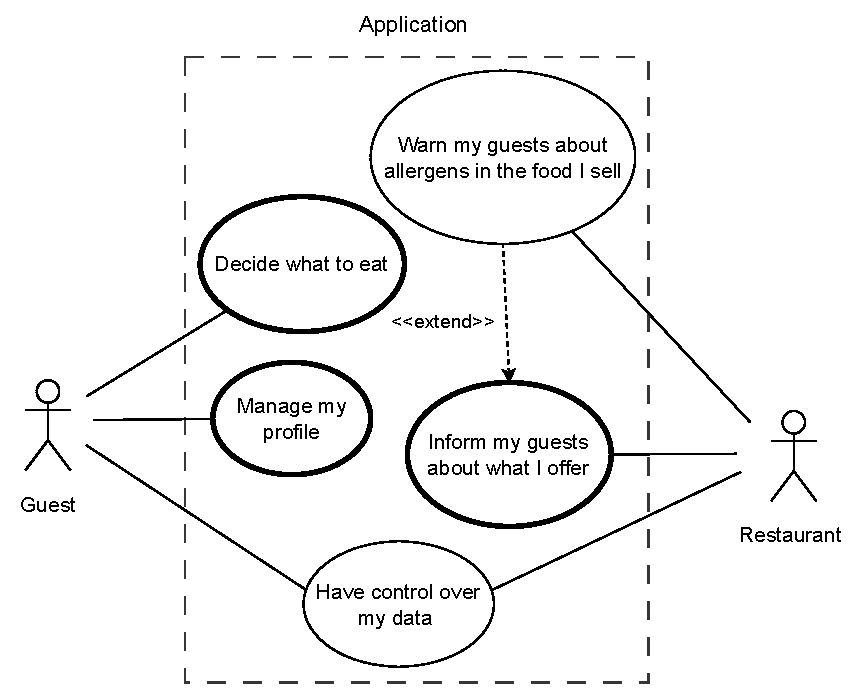
\includegraphics[width=\linewidth]{master-thesis/img/use_cases}
  \caption{The application's use case diagram.}
\end{figure}

\vspace*{\fill}

% Add top padding for scenario tables
\def\arraystretch{1.5}

\subsection{Guest use cases}

\begin{figure}[h]
  \centering
  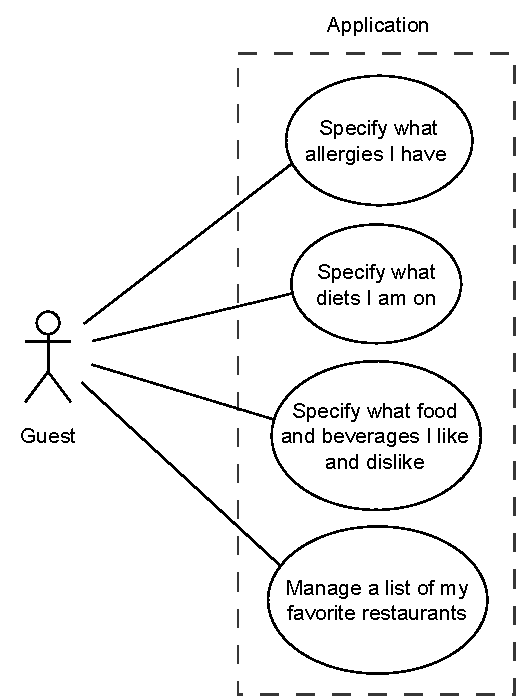
\includegraphics[width=0.62\linewidth]{master-thesis/img/use_cases_guest_profile_management}
  \caption{Guest profile management use cases}
\end{figure}

\noindent \textbf{1. Use case: Specify what allergies I have}
\begin{center}
  \begin{tabular}{| l | p{10.75cm} | }
    \hline
    Actor    & Guest \\
    \hline
    Scenario &
    \begin{minipage}[t]{\linewidth}
      \begin{enumerate}[leftmargin=*,nosep,before=\vspace{-0.575\baselineskip},after=\strut]
        \item The guest opens their profile.
        \item The guest selects a tab named "My allergies".
        \item The application displays a list of previously specified allergies by the guest. \textbf{A1}
        \item The guest clicks a button labeled "Add allergy".
        \item The application displays a search bar.
        \item The guest starts typing the name of an allergy into the search bar.
        \item The application suggests allergies which contain the given input in their name.
        \item The guest selects the desired allergy and clicks an "Add" button. \textbf{A2}
        \item The application adds the chosen allergy to the set of the guest's allergies. \textbf{A3}
        \item The guest repeats steps 4 to 9 until they have specified all their allergies.
      \end{enumerate}
    \end{minipage}
    \\
    \hline
    Alternatives &
    \begin{minipage}[t]{\linewidth}
      \begin{description}[nosep,after=\strut]
        \item [A1:] The list is empty because the guest has not specified any allergies yet. The application displays a text containing this information.
        \item [A2:] The application does not recognize the allergy which the guest is wishing to add. The guest creates an issue in the application's public repository with a request to add the desired allergy to the application.
        \item [A3:] The allergy the guest has chosen is already contained in the set of the guest's allergies. The application informs the guest about this fact and the set is not altered.
      \end{description}
    \end{minipage}
    \\
    \hline
  \end{tabular}
  \newline
\end{center}

\noindent \textbf{2. Use case: Specify what diets I am on}

\begin{center}
  \begin{tabular}{| l | p{10.75cm} | }
    \hline
    Actor    & Guest \\
    \hline
    Scenario &
    \begin{minipage}[t]{\linewidth}
      \begin{enumerate}[leftmargin=*,nosep,before=\vspace{-0.575\baselineskip},after=\strut]
        \item The guest opens their profile.
        \item The guest selects a tab named "My diets".
        \item The application displays a list of previously specified diets by the guest. \textbf{A1}
        \item The guest clicks a button labeled "Add diet".
        \item The application displays a search bar.
        \item The guest starts typing the name of a diet into the search bar.
        \item The application suggests diets which contain the given input in their name.
        \item The guest selects the desired diet and clicks an "Add" button. \textbf{A2}
        \item The application adds the chosen diet to the set of the guest's diets. \textbf{A3}
        \item The guest repeats steps 4 to 9 until they have specified all their diets.
      \end{enumerate}
    \end{minipage}
    \\
    \hline
    Alternatives &
    \begin{minipage}[t]{\linewidth}
      \begin{description}[nosep,after=\strut]
        \item [A1:] The list is empty because the guest has not specified any diets yet. The application displays a text containing this information.
        \item [A2:] The application does not recognize the diet which the guest is searching for. The guest creates an issue in the application's public repository with a request to add the desired diet to the application.
        \item [A3:] The diet the guest has chosen is already contained in the set of the guest's diets. The application informs the guest about this fact and the set is not altered.
      \end{description}
    \end{minipage}
    \\
    \hline
  \end{tabular}
  \newline
\end{center}

\noindent \textbf{7. Use case: Specify what food and beverages I like and dislike}

\begin{center}
  \begin{tabular}{| l | p{10.75cm} | }
    \hline
    Actor        & Guest \\
    \hline
    Scenario     &
    \begin{minipage}[t]{\linewidth}
      \begin{enumerate}[leftmargin=*,nosep,before=\vspace{-0.575\baselineskip},after=\strut]
        \item The guest opens their profile.
        \item The guest selects a tab named "My food preferences".
        \item The application displays two lists, one containing the foods which the guest likes and the other containing the foods which the guest dislikes. \textbf{A1}
        \item The guest clicks a button labeled as "Add food I like". \textbf{A2}
        \item The application provides a search bar with a text saying "Search foods...".
        \item The guest starts typing the name of the food.
        \item The application recommends foods from a predefined list which contain the given input text in their name.
        \item The guest selects the desired food and clicks an "Add" button. \textbf{A3}
        \item The application adds the chosen food to the guest's set of foods which they like. \textbf{A4}
      \end{enumerate}
    \end{minipage}
    \\
    \hline
    Alternatives &
    \begin{minipage}[t]{\linewidth}
      \begin{description}[nosep,after=\strut]
        \item [A1:] Either one or both of the lists can be empty if the guest has not specified any of their preferred or disliked foods yet. Instead of displaying a list, the application displays a text saying "No foods specified".
        \item [A2:] The guest clicks a button labeled "Add food I dislike". The use case continues with a difference that in the step number 9, the application adds the food to the guest's set of foods which they \emph{dislike}.
        \item [A3:] The guest is not able to find the food they are trying to select because the application does not recognize it. The guest writes an email to a special address with a request to add the desired food to the application.
        \item [A4:] The set already contains the food. The guest is informed about this fact and the set is not altered.
      \end{description}
    \end{minipage}
    \\
    \hline
  \end{tabular}
  \newline
\end{center}




\textbf{x. Use case: Find a meal I can eat at a restaurant}

\begin{center}
  \begin{tabular}{| l | p{10.75cm} | }
    \hline
    Actor        & Guest \\
    \hline
    Description  & A guest comes to a restaurant and is deciding what to order. \\
    \hline
    Scenario     &
    \begin{minipage}[t]{\linewidth}
      \begin{enumerate}[leftmargin=*,nosep,before=\vspace{-0.575\baselineskip},after=\strut]
        \item The guest scans a QR code on a printed menu which takes him to the application.
        \item The application loads and displays the online version of the menu.
        \item The guest selects that they wish to filter out meals of the menu which do not correspond to their profile preferences. \textbf{A1}
        \item The guest chooses a meal from the personalized menu.
      \end{enumerate}
    \end{minipage}
    \\
    \hline
    Alternatives &
    \begin{minipage}[t]{\linewidth}
      \begin{description}[nosep,after=\strut]
        \item [A1:] The guest selects that they wish to sort the menu according to their profile preferences.
      \end{description}
    \end{minipage}
    \\
    \hline
  \end{tabular}
  \newline
\end{center}

\noindent \textbf{2. Use case: Manage a list of my favorite restaurants}

\begin{center}
  \begin{tabular}{| l | p{10.75cm} | }
    \hline
    Actor        & Guest \\
    \hline
    Scenario     &
    \begin{minipage}[t]{\linewidth}
      \begin{enumerate}[leftmargin=*,nosep,before=\vspace{-0.575\baselineskip},after=\strut]
        \item The guest selects a tab named "Manage my favorite restaurants".
        \item The application displays a screen with infor
        \item The guest specifies the IRI of the restaurant which they wish to add to the list of their favorite restaurants. \textbf{A1}
        \item The application displays the restaurant's detail. 
        \item The guest clicks a heart icon next to the restaurant's name.
        \item The application adds the restaurant to the list of the guest's favorite restaurants.
      \end{enumerate}
    \end{minipage}
    \\
    \hline
    Alternatives &
    \begin{minipage}[t]{\linewidth}
      \begin{description}[nosep,after=\strut]
        \item [A1:] The guest opens their profile and adds the restaurant to the list of their favorite restaurants manually.
      \end{description}
    \end{minipage}
    \\
    \hline
  \end{tabular}
  \newline
\end{center}

\noindent \textbf{3. Use case: Look up online what a restaurant offers today}

\begin{center}
  \begin{tabular}{| l | p{10.75cm} | }
    \hline
    Actor        & Guest \\
    \hline
    Description  & A guest is at home or on their way to a restaurant and wants to know what the restaurant serves at the moment. \\
    \hline
    Scenario     &
    \begin{minipage}[t]{\linewidth}
      \begin{enumerate}[leftmargin=*,nosep,before=\vspace{-0.575\baselineskip},after=\strut]
        \item The guest clicks a button labeled "Find restaurant by IRI". \textbf{A1}
        \item The application provides a text input field.
        \item The guest specifies the IRI of the restaurant in the provided input field and clicks a "Find" button.
        \item The application displays the detail of the restaurant. \textbf{A2}
        \item The guest clicks a button labeled "Detail" next to the menu which they wish to view.
        \item The application displays the chosen menu.
      \end{enumerate}
    \end{minipage}
    \\
    \hline
    Alternatives &
    \begin{minipage}[t]{\linewidth}
      \begin{description}[nosep,after=\strut]
        \item [A1:] The guest opens a tab named "My favorite restaurants". The application displays the list of the guest's favorite restaurants. The guest clicks a "Detail" button next to the desired restaurant. The guest continues with step 5.
        \item [A2:] The application could not find the restaurant by the specified IRI and informs the guest about it by displaying an error page.
      \end{description}
    \end{minipage}
    \\
    \hline
  \end{tabular}
  \newline
\end{center}

\noindent \textbf{4. Use case: Find currently served meals by my favorite restaurants which correspond to my profile}

\begin{center}
  \begin{tabular}{| l | p{10.75cm} | }
    \hline
    Actor        & Guest \\
    \hline
    Description  & A guest is at home or at work and wants to see what do their favorite restaurants currently have to offer. \\
    \hline
    Scenario     &
    \begin{minipage}[t]{\linewidth}
      \begin{enumerate}[leftmargin=*,nosep,before=\vspace{-0.575\baselineskip},after=\strut]

        \item The application shows currently valid menus of the guest's favorite restaurants by default. A1 A2 - currently no meals are served A3 meals are served but none correspond to profile
      \end{enumerate}
    \end{minipage}
    \\
    \hline
    Alternatives &
    \begin{minipage}[t]{\linewidth}
      \begin{description}[nosep,after=\strut]
        \item [A1:] The guest has no restaurants in their list of favorite restaurants. The application displays a screen with instructions on how to add a restaurant to the list.
        \item [A2:] The restaurants in the guest's list of favorite restaurants have no menus uploaded which are valid at the moment. The application displays a screen which says 

        zobrazit restauracie
        zobrazit jedla
      
      \end{description}
    \end{minipage}
    \\
    \hline
  \end{tabular}
  \newline
\end{center}

\noindent \textbf{x. Use case: Specify where should the application store my data}

\begin{center}
  \begin{tabular}{| l | p{10.75cm} | }
    \hline
    Actor        & Restaurant \\
    \hline
    Description  &  \\
    \hline
    Scenario     &
    \begin{minipage}[t]{\linewidth}
      \begin{enumerate}[leftmargin=*,nosep,before=\vspace{-0.575\baselineskip},after=\strut]
        \item ...
        \item ... \textbf{A1}
        \item ...
      \end{enumerate}
    \end{minipage}
    \\
    \hline
    Alternatives &
    \begin{minipage}[t]{\linewidth}
      \begin{description}[nosep,after=\strut]
        \item [A1:] ...
      \end{description}
    \end{minipage}
    \\
    \hline
  \end{tabular}
  \newline
\end{center}

\subsection{Restaurant use cases}

\noindent \textbf{8. Use case: Post a menu online}

\begin{center}
  \begin{tabular}{| l | p{10.75cm} | }
    \hline
    Actor        & Restaurant \\
    \hline
    Description  & A restaurant's management decides to post their currently valid menu online. \\
    \hline
    Scenario     &
    \begin{minipage}[t]{\linewidth}
      \begin{enumerate}[leftmargin=*,nosep,before=\vspace{-0.575\baselineskip},after=\strut]
        \item The restaurant employee creates the menu as in the use case x.
        \item The application generates a URL which points to the application, providing it with the created menu.
        \item The restaurant employee adds the generated URL to the restaurant's webpage. \textbf{A1}
      \end{enumerate}
    \end{minipage}
    \\
    \hline
    Alternatives &
    \begin{minipage}[t]{\linewidth}
      \begin{description}[nosep,after=\strut]
        \item [A1:] The restaurant employee shares the generated URL on the restaurant's social media.
      \end{description}
    \end{minipage}
    \\
    \hline
  \end{tabular}
  \newline
\end{center}

\noindent \textbf{9. Use case: Allow my guests to view a menu by scanning a QR code}

\begin{center}
  \begin{tabular}{| l | p{10.75cm} |}
    \hline
    Actor        & Restaurant \\
    \hline
    Description  & A restaurant's management would like to provide a menu with a QR code which will take the restaurant's guests to the application. \\
    \hline
    Scenario     &
    \begin{minipage}[t]{\linewidth}
      \begin{enumerate}[leftmargin=*,nosep,before=\vspace{-0.575\baselineskip},after=\strut]
        \item The restaurant employee creates a menu as in use case x, ensuring that a checkbox labeled "Add a QR code" is checked. \textbf{A1}
        \item The application generates a QR code which will link a guest to the application.
        \item The restaurant employee prints the menu and puts in on tables as in use case x.
        \item A guest scans the QR code on the printed menu.
        \item The application displays the menu.
      \end{enumerate}
    \end{minipage}
    \\
    \hline
    Alternatives &
    \begin{minipage}[t]{\linewidth}
      \begin{description}[nosep,after=\strut]
        \item [A1:] The restaurant employee selects a menu from previously created menus.
      \end{description}
    \end{minipage}
    \\
    \hline
  \end{tabular}
  \newline
\end{center}

\noindent \textbf{10. Use case: Change an ingredient of a meal in an existing menu}

\begin{center}
  \begin{tabular}{| l | p{10.75cm} | }
    \hline
    Actor        & Restaurant \\
    \hline
    Scenario     &
    \begin{minipage}[t]{\linewidth}
      \begin{enumerate}[leftmargin=*,nosep,before=\vspace{-0.575\baselineskip},after=\strut]
        \item The restaurant employee logs in to the application.
        \item The restaurant employee clicks an "Edit" button next to a menu.
        \item The application lets the restaurant employee edit the menu.
      \end{enumerate}
    \end{minipage}
    \\
    % \hline
    % Alternatives &
    % \begin{minipage}[t]{\linewidth}
    %   \begin{description}[nosep,after=\strut]
    %     \item [A1:] ...
    %   \end{description}
    % \end{minipage}
    % \\
    \hline
  \end{tabular}
  \newline
\end{center}

\noindent \textbf{11. Use case: Place a menu on tables}

\begin{center}
  \begin{tabular}{| l | p{10.75cm} | }
    \hline
    Actor        & Restaurant \\
    \hline
    Description  & A restaurant employee would like to print a menu and place it on tables. \\
    \hline
    Scenario     &
    \begin{minipage}[t]{\linewidth}
      \begin{enumerate}[leftmargin=*,nosep,before=\vspace{-0.575\baselineskip},after=\strut]
        \item The restaurant employee logs in to the application.
        \item The restaurant employee creates a new menu. \textbf{A1}
        \item The application displays a detail of the menu.
        \item The restaurant employee clicks a "Print" button in the detail of the menu.
        \item The application manages to print the menu.
      \end{enumerate}
    \end{minipage}
    \\
    \hline
    Alternatives &
    \begin{minipage}[t]{\linewidth}
      \begin{description}[nosep,after=\strut]
        \item [A1:] The restaurant employee selects an existing menu and proceeds with step 3.
      \end{description}
    \end{minipage}
    \\
    \hline
  \end{tabular}
  \newline
\end{center}

\noindent \textbf{13. Use case: Reuse an existing daily menu for today.}

\begin{center}
  \begin{tabular}{| l | p{10.75cm} | }
    \hline
    Actor        & Restaurant \\
    \hline
    Description  &  \\
    \hline
    Scenario     &
    \begin{minipage}[t]{\linewidth}
      \begin{enumerate}[leftmargin=*,nosep,before=\vspace{-0.575\baselineskip},after=\strut]
        \item The restaurant employee logs in to the application.
        \item The restaurant employee clicks a button labeled "Create new menu". \textbf{A1}
        \item The application asks the restaurant employee what kind of menu they would like to create.
        \item The restaurant employee selects that they wish to create a daily menu.
        \item The application asks the restaurant employee whether they want to use an existing menu as a template.
        \item The restaurant employee confirms by clicking a "Yes" button.
        \item The application displays a list of menus as possible templates.
        \item The restaurant employee chooses a menu from the list.
        \item The application loads the chosen menu.
        \item The restaurant employee changes the date of validity of the menu.
        \item The restaurant employee clicks a "Save menu" button.
        \item The application asks the restaurant employee whether they would like to overwrite the existing menu.
        \item The restaurant employee denies by clicking a "No, create a new menu" button. \textbf{A2}
        \item The application saves the menu.
      \end{enumerate}
    \end{minipage}
    \\
    \hline
    Alternatives &
    \begin{minipage}[t]{\linewidth}
      \begin{description}[nosep,after=\strut]
        \item [A1:] The restaurant employee clicks an "Edit" button next to a menu which they want to reuse. The restaurant employee edits a date field which controls for which day the menu is valid. The restaurant employee then clicks a "Save menu" button and the application saves the menu.
        \item [A2:] The restaurant employee confirms by clicking a "Yes" button and the application overwrites the old menu with the new one.
      \end{description}
    \end{minipage}
    \\
    \hline
  \end{tabular}
  \newline
\end{center}

\begin{figure}[h]
  \centering
  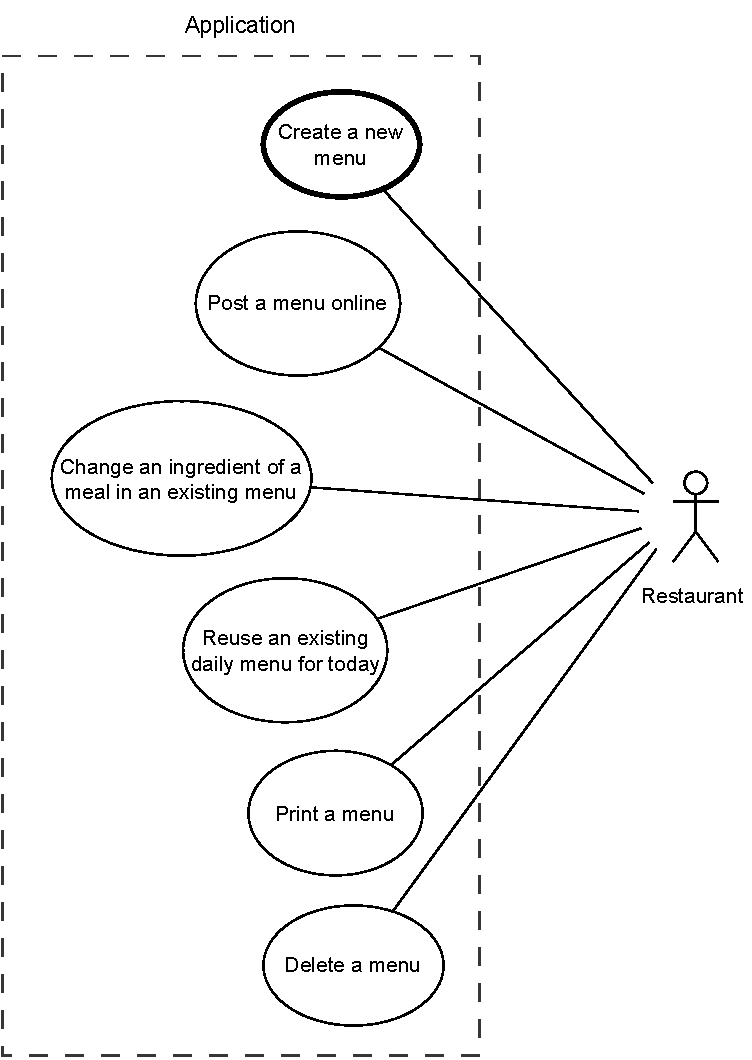
\includegraphics[width=0.62\linewidth]{master-thesis/img/use_cases_restaurant_menu_management}
  \caption{Restaurant menu creation use cases}
\end{figure}

\noindent \textbf{14. Use case: Specify allergens contained in an item of a menu}

\begin{center}
  \begin{tabular}{| l | p{10.75cm} | }
    \hline
    Actor        & Restaurant \\
    \hline
    Description  &  \\
    \hline
    Scenario     &
    \begin{minipage}[t]{\linewidth}
      \begin{enumerate}[leftmargin=*,nosep,before=\vspace{-0.575\baselineskip},after=\strut]
        \item ...
        \item ... \textbf{A1}
        \item ...
      \end{enumerate}
    \end{minipage}
    \\
    \hline
    Alternatives &
    \begin{minipage}[t]{\linewidth}
      \begin{description}[nosep,after=\strut]
        \item [A1:] ...
      \end{description}
    \end{minipage}
    \\
    \hline
  \end{tabular}
  \newline
\end{center}

\noindent \textbf{15. Use case: Specify items of a menu}

\begin{center}
  \begin{tabular}{| l | p{10.75cm} | }
    \hline
    Actor        & Restaurant \\
    \hline
    Description  &  \\
    \hline
    Scenario     &
    \begin{minipage}[t]{\linewidth}
      \begin{enumerate}[leftmargin=*,nosep,before=\vspace{-0.575\baselineskip},after=\strut]
        \item ...
        \item ... \textbf{A1}
        \item ...
      \end{enumerate}
    \end{minipage}
    \\
    \hline
    Alternatives &
    \begin{minipage}[t]{\linewidth}
      \begin{description}[nosep,after=\strut]
        \item [A1:] ...
      \end{description}
    \end{minipage}
    \\
    \hline
  \end{tabular}
  \newline
\end{center}

\noindent \textbf{16. Use case: Create a daily menu for tomorrow}

\begin{center}
  \begin{tabular}{| l | p{10.75cm} | }
    \hline
    Actor        & Restaurant \\
    \hline
    Scenario     &
    \begin{minipage}[t]{\linewidth}
      \begin{enumerate}[leftmargin=*,nosep,before=\vspace{-0.575\baselineskip},after=\strut]
        \item The restaurant employee logs in to the application.
        \item The restaurant employee clicks a button labeled "Create new menu".
        \item The application asks the restaurant employee what kind of menu they would like to create.
        \item The restaurant employee chooses that they wish to create a daily menu.
        \item The application asks the restaurant employee whether they want to use an existing menu as a template.
        \item The restaurant employee denies by clicking a "No, create a new menu" button.
        \item The restaurant employee specifies items of the menu.
        \item The restaurant employee specifies which day the menu will be valid.
        \item The restaurant employee clicks a "Save menu" button.
        \item The application saves the menu.
      \end{enumerate}
    \end{minipage}
    \\
    \hline
    % Alternatives &
    % \begin{minipage}[t]{\linewidth}
    %   \begin{description}[nosep,after=\strut]
    %     \item [A1:] ...
    %   \end{description}
    % \end{minipage}
    % \\
    % \hline
  \end{tabular}
  \newline
\end{center}

\noindent \textbf{17. Use case: Specify allergens contained in a meal}

\begin{center}
  \begin{tabular}{| l | p{10.75cm} | }
    \hline
    Actor        & Restaurant \\
    \hline
    Scenario     &
    \begin{minipage}[t]{\linewidth}
      \begin{enumerate}[leftmargin=*,nosep,before=\vspace{-0.575\baselineskip},after=\strut]
        \item The restaurant employee logs in to the application.
        \item The restaurant employee clicks a "Create a menu" button.
        \item The application asks the restaurant employee what kind of menu they would like to create.
        \item The restaurant employee selects one of the options.
        \item The restaurant employee clicks a plus sign on the new menu to add an item to it.
        \item The restaurant employee adds information about the food item.
        \item The application gives the restaurant employee a list of all allergens. \textbf{A1}
        \item The restaurant employee selects allergens which are contained in the meal.
        \item The restaurant employee clicks a "Save menu" button.
        \item The application saves the menu.
      \end{enumerate}
    \end{minipage}
    \\
    \hline
    Alternatives &
    \begin{minipage}[t]{\linewidth}
      \begin{description}[nosep,after=\strut]
        \item [A1:] The restaurant employee starts typing the name of an ingredient. The application provides predefined ingredients and automatically adds allergens contained in the selected ingredient as the food item's allergens. The restaurant employee then continues with step 9.
      \end{description}
    \end{minipage}
    \\
    \hline
  \end{tabular}
  \newline
\end{center}

\noindent \textbf{18. Use case: Create a daily menu which will repeat each Tuesday}

\begin{center}
  \begin{tabular}{| l | p{10.75cm} | }
    \hline
    Actor        & Restaurant \\
    \hline
    Description  &  \\
    \hline
    Scenario     &
    \begin{minipage}[t]{\linewidth}
      \begin{enumerate}[leftmargin=*,nosep,before=\vspace{-0.575\baselineskip},after=\strut]
        \item The restaurant employee logs in to the application.
        \item The restaurant employee clicks a button labeled "Create new menu". 
        \item The application asks the restaurant employee what kind of menu they would like to create.
        \item The restaurant employee chooses that they wish to create a daily menu.
        \item The application asks the restaurant employee whether they want to use an existing menu as a template.
        \item The restaurant employee denies by clicking a "No, create a new menu" button.
        \item The restaurant employee specifies items of the menu.
        \item The restaurant employee specifies that the menu will be valid the next Tuesday.
        \item The restaurant employee ensures that a checkbox labeled "Repeat every week" is checked.
        \item The restaurant employee clicks a "Save menu" button.
        \item The application saves the menu.
      \end{enumerate}
    \end{minipage}
    \\
    \hline
    % Alternatives &
    % \begin{minipage}[t]{\linewidth}
    %   \begin{description}[nosep,after=\strut]
    %     \item [A1:] 
    %   \end{description}
    % \end{minipage}
    % \\
    % \hline
  \end{tabular}
  \newline
\end{center}

\noindent \textbf{19. Use case: Create a stable menu}

\begin{center}
  \begin{tabular}{| l | p{10.75cm} | }
    \hline
    Actor        & Restaurant \\
    \hline
    Description  & A restaurant's management wants its restaurant to have a stable menu which will be valid every day. \\
    \hline
    Scenario     &
    \begin{minipage}[t]{\linewidth}
      \begin{enumerate}[leftmargin=*,nosep,before=\vspace{-0.575\baselineskip},after=\strut]
        \item The restaurant employee logs in to the application.
        \item The restaurant employee clicks a button labeled "Create new menu". 
        \item The application asks the restaurant employee what kind of menu they would like to create.
        \item The restaurant employee chooses that they wish to create a stable menu.
        \item The restaurant employee specifies items of the menu.
        \item The restaurant employee clicks a "Save menu" button.
        \item The application saves the menu.
      \end{enumerate}
    \end{minipage}
    \\
    \hline
    % Alternatives &
    % \begin{minipage}[t]{\linewidth}
    %   \begin{description}[nosep,after=\strut]
    %     \item [A1:] ...
    %   \end{description}
    % \end{minipage}
    % \\
    % \hline
  \end{tabular}
  \newline
\end{center}

\noindent \textbf{20. Use case: Create daily menus for the next week}

\begin{center}
  \begin{tabular}{| l | p{10.75cm} | }
    \hline
    Actor        & Restaurant \\
    \hline
    Description  &  \\
    \hline
    Scenario     &
    \begin{minipage}[t]{\linewidth}
      \begin{enumerate}[leftmargin=*,nosep,before=\vspace{-0.575\baselineskip},after=\strut]
        \item The restaurant employee logs in to the application.
        \item The restaurant employee clicks a button labeled "Create new menu".
        \item The application asks the restaurant employee what kind of menu they would like to create.
        \item The restaurant employee chooses that they wish to create a daily menu.
        \item The restaurant employee specifies items of the menu.
        \item The restaurant employee specifies which day the menu will be valid.
        \item The restaurant employee clicks a "Save menu" button.
        \item The application saves the menu.
        \item The restaurant employee begins again with step 2 until menus for the whole week are created.
      \end{enumerate}
    \end{minipage}
    \\
    \hline
    % Alternatives &
    % \begin{minipage}[t]{\linewidth}
    %   \begin{description}[nosep,after=\strut]
    %     \item [A1:] ...
    %   \end{description}
    % \end{minipage}
    % \\
    % \hline
  \end{tabular}
  \newline
\end{center}

\noindent \textbf{21. Use case: Create a list of beverages}

\begin{center}
  \begin{tabular}{| l | p{10.75cm} | }
    \hline
    Actor        & Restaurant \\
    \hline
    Description  &  \\
    \hline
    Scenario     &
    \begin{minipage}[t]{\linewidth}
      \begin{enumerate}[leftmargin=*,nosep,before=\vspace{-0.575\baselineskip},after=\strut]
        \item The restaurant employee logs in to the application.
        \item The restaurant employee clicks a button labeled "Create new menu". 
        \item The application asks the restaurant employee what kind of menu they would like to create.
        \item The restaurant employee chooses that they wish to create a list of beverages.
        \item The restaurant employee specifies beverages of the menu.
        \item The restaurant employee clicks a "Save menu" button.
        \item The application saves the menu.
      \end{enumerate}
    \end{minipage}
    \\
    \hline
    % Alternatives &
    % \begin{minipage}[t]{\linewidth}
    %   \begin{description}[nosep,after=\strut]
    %     \item [A1:] ...
    %   \end{description}
    % \end{minipage}
    % \\
    % \hline
  \end{tabular}
  \newline
\end{center}

\noindent \textbf{22. Use case: Create a stable menu in a foreign language}

\begin{center}
  \begin{tabular}{| l | p{10.75cm} | }
    \hline
    Actor        & Restaurant \\
    \hline
    Description  & A restaurant's management wishes to have \\
    \hline
    Scenario     &
    \begin{minipage}[t]{\linewidth}
      \begin{enumerate}[leftmargin=*,nosep,before=\vspace{-0.575\baselineskip},after=\strut]
        \item The restaurant employee logs in to the application.
        \item The restaurant employee clicks a button labeled "Create new menu". 
        \item The application asks the restaurant employee what kind of menu they would like to create.
        \item The restaurant employee selects that they wish to create a stable menu.

        \item The restaurant employee selects what currency to use in the menu.
        \item The restaurant employee selects what weight measurement units to use in the menu.

        \item The restaurant employee clicks a button labeled "Add category".
        \item The application displays a screen for adding a new category.
        \item The restaurant employee specifies the name of a new category of the menu in the foreign language.
        \item The restaurant employee clicks an "Add" button.
        \item The application adds the category to the menu.
        \item The restaurant employee repeats steps x to y until they have created all categories of the new menu.
        
        \item The restaurant employee clicks an "Add item" button.
        \item The application asks the restaurant employee whether they would like to add a meal or a drink to the menu.
        \item The restaurant employee selects that they wish to add a meal to the menu. A1 drink
        \item The application displays a screen for adding a new meal to the menu.
        \item The restaurant employee specifies the meal's name in the foreign language.
        \item The restaurant employee specifies the meal's price and weight.
        \item The restaurant employee clicks a button labeled "Add ingredient".
        \item The application provides a list of possible ingredients.
        \item The restaurant employee selects an ingredient from the list and clicks "Add".
        \item The restaurant employee repeats steps x to y until all ingredients of the meal are added.
        \item The restaurant employee clicks a button labeled "Add allergen". A2 - the application fills allergens contained in the ingredient automatically based on the provided ingredient
        \item The application provides a list of possible allergens.
        \item The restaurant employee selects an allergen from the list and clicks "Add".
        \item The restaurant employee repeats steps x to y until all allergens of the meal are specified.
        \item The restaurant employee repeats steps x to y until they have specified all items of the menu.

        \item The restaurant employee clicks a "Save menu" button.
        \item The application saves the menu.
      \end{enumerate}
    \end{minipage}
    \\
    \hline
    Alternatives &
    \begin{minipage}[t]{\linewidth}
      \begin{description}[nosep,after=\strut]
        \item [A1:] ...
      \end{description}
    \end{minipage}
    \\
    \hline
  \end{tabular}
  \newline
\end{center}

\noindent \textbf{x. Use case: Create a new menu}

\begin{center}
  \begin{tabular}{| l | p{10.75cm} | }
    \hline
    Actor        & Restaurant \\
    \hline
    Scenario     &
    \begin{minipage}[t]{\linewidth}
      \begin{enumerate}[leftmargin=*,nosep,before=\vspace{-0.575\baselineskip},after=\strut]
        \item The restaurant employee clicks a button labeled "Create new menu". 
        \item The application displays a screen for creating a new menu.
        \item The restaurant employee creates categories of the new menu. \textbf{A1}
        \item The restaurant employee specifies items, along with allergens contained in them, and assign them to the categories of the new menu.
        \item The restaurant employee clicks a "Save" button and the application saves the menu.
      \end{enumerate}
    \end{minipage}
    \\
    \hline
    Alternatives &
    \begin{minipage}[t]{\linewidth}
      \begin{description}[nosep,after=\strut]
        \item [A1:] The restaurant employee skips the creation of categories and only specifies the items of the menu. The restaurant employee then continues with step 5.
      \end{description}
    \end{minipage}
    \\
    \hline
  \end{tabular}
  \newline
\end{center}

\noindent \textbf{x. Use case: Select what currency to use in a menu}

\begin{center}
  \begin{tabular}{| l | p{10.75cm} | }
    \hline
    Actor        & Restaurant \\
    \hline
    Description  & A restaurant employee has created an empty menu and wants to set what currency to use in a menu. \\
    \hline
    Scenario     &
    \begin{minipage}[t]{\linewidth}
      \begin{enumerate}[leftmargin=*,nosep,before=\vspace{-0.575\baselineskip},after=\strut]
        \item The restaurant employee clicks a button labeled "Choose currency for the menu".
        \item The application provides a predefined list of currencies. 
        \item The restaurant employee selects the desired currency and clicks an "Ok" button.
        \item The application sets the selected currency for the menu.
      \end{enumerate}
    \end{minipage}
    \\
    \hline
  \end{tabular}
  \newline
\end{center}

\noindent \textbf{x. Use case: Select what weight units to use in a menu}

\begin{center}
  \begin{tabular}{| l | p{10.75cm} | }
    \hline
    Actor        & Restaurant \\
    \hline
    Description  & A restaurant employee has created an empty menu and wants to set what weight units to use in it. \\
    \hline
    Scenario     &
    \begin{minipage}[t]{\linewidth}
      \begin{enumerate}[leftmargin=*,nosep,before=\vspace{-0.575\baselineskip},after=\strut]
        \item The restaurant employee clicks a button labeled "Choose weight units".
        \item The application provides a predefined set of weight units.
        \item The restaurant employee selects the desired weight unit and clicks an "Ok" button.
        \item The application sets the selected weight unit for the menu.
      \end{enumerate}
    \end{minipage}
    \\
    \hline
  \end{tabular}
  \newline
\end{center}

\noindent \textbf{x. Use case: Add a category to a menu}

\begin{center}
  \begin{tabular}{| l | p{10.75cm} | }
    \hline
    Actor        & Restaurant \\
    \hline
    Description  & A restaurant employee has created an empty menu and wants to add a category to it. \\
    \hline
    Scenario     &
    \begin{minipage}[t]{\linewidth}
      \begin{enumerate}[leftmargin=*,nosep,before=\vspace{-0.575\baselineskip},after=\strut]
        \item The restaurant employee clicks a button labeled "Add category".
        \item The restaurant employee specifies the name of the category.
        \item The application adds the category to the menu.
      \end{enumerate}
    \end{minipage}
    \\
    \hline
  \end{tabular}
  \newline
\end{center}

\noindent \textbf{x. Use case: Specify allergens contained in an item of a menu}

\begin{center}
  \begin{tabular}{| l | p{10.75cm} | }
    \hline
    Actor        & Restaurant \\
    \hline
    Description  & A restaurant's employee is creating a menu. They have added an item to the menu and want to specify allergens contained in it. \\
    \hline
    Scenario     &
    \begin{minipage}[t]{\linewidth}
      \begin{enumerate}[leftmargin=*,nosep,before=\vspace{-0.575\baselineskip},after=\strut]
        \item The restaurant employee clicks a button labeled "Add allergen". \textbf{A1}
        \item The application provides a predefined list of possible allergens.
        \item The restaurant employee selects an allergen from the list and clicks "Add".
        \item The restaurant employee repeats steps x to y until all allergens of the item are added.
      \end{enumerate}
    \end{minipage}
    \\
    \hline
    Alternatives &
    \begin{minipage}[t]{\linewidth}
      \begin{description}[nosep,after=\strut]
        \item [A1:] The application adds allergens contained in the ingredient automatically based on the provided ingredient (see x. Use case: Add an item to a menu).
      \end{description}
    \end{minipage}
    \\
    \hline
  \end{tabular}
  \newline
\end{center}

\noindent \textbf{x. Use case: Add an item to a menu}

\begin{center}
  \begin{tabular}{| l | p{10.75cm} | }
    \hline
    Actor        & Restaurant \\
    \hline
    Description  & A restaurant's employee has created an empty menu and wants to add an item to it. \\
    \hline
    Scenario     &
    \begin{minipage}[t]{\linewidth}
      \begin{enumerate}[leftmargin=*,nosep,before=\vspace{-0.575\baselineskip},after=\strut]
        \item The restaurant employee clicks an "Add item" button.
        \item The application displays a screen for adding an item to a menu.
        \item The restaurant employee specifies the item's name, price and amount.
        \item The restaurant employee clicks a button labeled "Add ingredient".
        \item The application provides a predefined list of ingredients.
        \item The restaurant employee selects an ingredient from the list and clicks "Add". \textbf{A1}
        \item The restaurant employee repeats steps x to y until all ingredients of the item are added.
        \item The restaurant employee adds allergens contained in the item (see x. Use case: Specify allergens contained in an item of a menu).
      \end{enumerate}
    \end{minipage}
    \\
    \hline
    Alternatives &
    \begin{minipage}[t]{\linewidth}
      \begin{description}[nosep,after=\strut]
        \item [A1:] The restaurant employee also specifies the amount of the ingredient contained in the item. The restaurant employee continues with step x.
      \end{description}
    \end{minipage}
    \\
    \hline
  \end{tabular}
  \newline
\end{center}

\noindent \textbf{x. Use case: Add my restaurant's information to a menu}

\begin{center}
  \begin{tabular}{| l | p{10.75cm} | }
    \hline
    Actor        & Restaurant \\
    \hline
    Description  & A restaurant's employee has created an empty menu and wants to add basic information about the restaurant. \\
    \hline
    Scenario     &
    \begin{minipage}[t]{\linewidth}
      \begin{enumerate}[leftmargin=*,nosep,before=\vspace{-0.575\baselineskip},after=\strut]
        \item The restaurant employee clicks a button labeled "Add restaurant information".
        \item The application displays a screen for adding basic restaurant information.
        \item The restaurant employee specifies the restaurant's name, address and phone number.
        \item The restaurant employee clicks an "Add" button.
        \item The application adds the specified information to the menu. 
      \end{enumerate}
    \end{minipage}
    \\
    \hline
  \end{tabular}
  \newline
\end{center}

\noindent \textbf{x. Use case: Specify where should the application store my data }

\begin{center}
  \begin{tabular}{| l | p{10.75cm} | }
    \hline
    Actor        & Restaurant \\
    \hline
    Description  &  \\
    \hline
    Scenario     &
    \begin{minipage}[t]{\linewidth}
      \begin{enumerate}[leftmargin=*,nosep,before=\vspace{-0.575\baselineskip},after=\strut]
        \item ...
        \item ... \textbf{A1}
        \item ...
      \end{enumerate}
    \end{minipage}
    \\
    \hline
    Alternatives &
    \begin{minipage}[t]{\linewidth}
      \begin{description}[nosep,after=\strut]
        \item [A1:] ...
      \end{description}
    \end{minipage}
    \\
    \hline
  \end{tabular}
  \newline
\end{center}